\begin{figure*}[ht]
    \caption{The sequence diagram of the OTP wallet. After initialization, the OTP device
             becomes air gapped and the user submits the OTP visually to an online computer
             at time $t$.}
    \centering
    \iflncs
        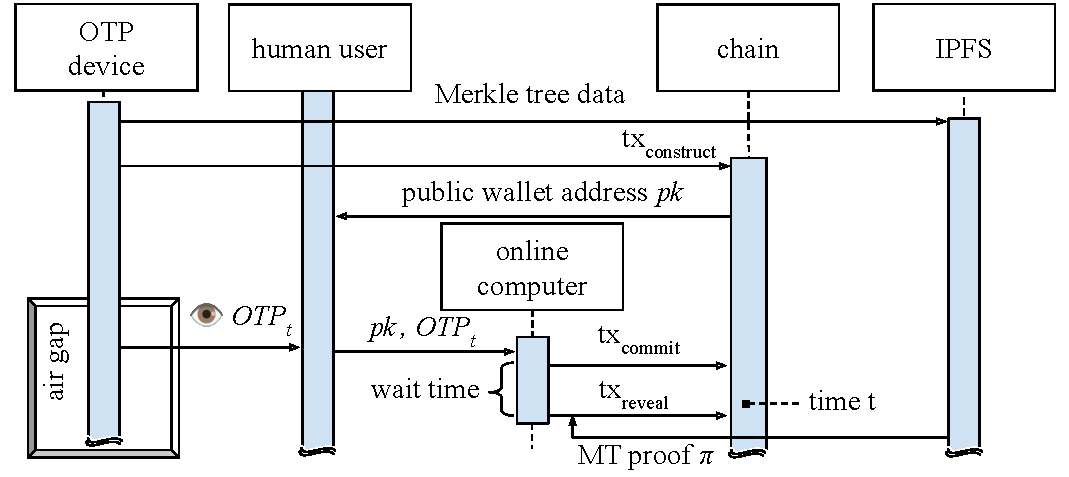
\includegraphics[width=\textwidth,keepaspectratio]{figures/otp-sequence-diagram.pdf}
    \else
        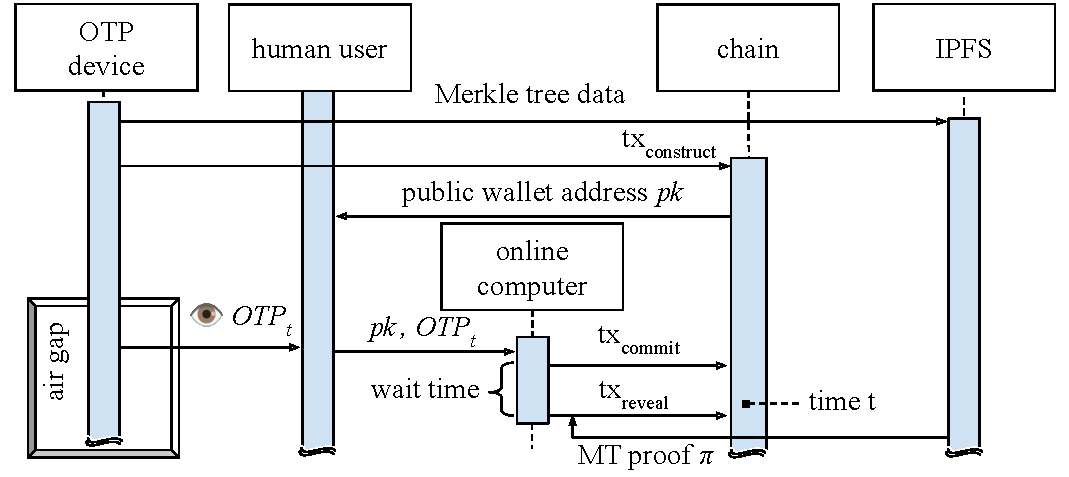
\includegraphics[width=0.7 \textwidth,keepaspectratio]{figures/otp-sequence-diagram.pdf}
    \fi
    \label{fig.sequence-diagram}
\end{figure*}

\section{An OTP Wallet}

The previous password-based construction has an important limitaton:
The money can only be spent once and at a prespecified date. This makes
the wallet highly unusable in practice.

Using the previous construction as a stepping stone,
we now move on to describe our \emph{Hours of Horus} scheme.
This is an OTP-based scheme in which the OTP is used as the \emph{single factor}
for wallet access, without any need to use private keys for signing.

The workflow of the OTP wallet is illustrated as a sequence diagram
in Figure~\ref{fig.sequence-diagram}. At the beginning, Alice initializes
a time-based OTP device (such as a mobile phone app) which
generates and stores an OTP seed (leftmost column). Upon this generation, the device also
generates a smart contract, which is constructed and submitted to the chain
through a transaction $\textsf{tx}_\textsf{construct}$, as in the construction of
Section~\ref{sec:password}. This transaction generates a wallet address $pk$ to which
payers can send money for Alice. The OTP device also constructs a Merkle tree containing
a large number of encrypted future OTPs and submits them to IPFS~\cite{ipfs} (or other persistent storage service)
publicly for availability reasons (rightmost column). These data could also be submitted to the chain, if
gas costs allow. Both $pk$ and all internal Merkle tree nodes are public. After this
initial phase, the OTP device becomes air gapped.

At any time Alice wishes to spend, she visually consults her OTP device which displays a time-based
OTP key. Using a (newly booted) online computer, she creates a transaction $\textsf{tx}_\textsf{commit}$ in
which she commits to the $OTP$, the amount she wishes to spend, and the target address.
The wallet waits a short amount of time before submitting the final $\textsf{tx}_\textsf{reveal}$
to confirm the spending. This transaction is accompanied by a Merkle tree proof-of-inclusion
constructed using the IPFS data. The wallet then releases the payment to the desired address.

Let us now give the technical details of how these transactions are constructed.
The smart contract deployed as a wallet is illustrated in Algorithm~\ref{alg.otp}.
The interaction with the smart contract by the user is illustrated in Algorithm~\ref{alg.otp.external}.
The constructor method of the smart contract accepts a parameter $r$
denoting a root of a Merkle tree. This is constructed by generating a large number ($\textsf{MAX\_TIME}$)
of time-based OTPs for the foreseeable future. For example, to support a wallet with
a lifetime of $100$ years with an hourly OTP resolution, $876{,}000$ codes need to
be generated. Let ${OTP}_t$ denote the OTP for future time $t \in \mathbb{N}$ (in
the example, $t$ would range from $1$ to $876{,}000$). These are generated from
the OTP seed in the OTP device by invoking the pseudorandom function
$\mathcal{G}(\textsf{seed}, t)$ whose output has $\lambda$ bits of entropy.
Each such OTP is then timelock encrypted for time $t$, multiplied by the expected
hourly production rate of the blockchain (the \emph{hourly} resolution is an arbitrary
choice that can be made differently, giving rise to a tradeoff between how much
data must be stored on IPFS versus how often the user can spend her money).
Specifically, the software computes $c_t = \textsf{timelock}(\textsf{OTP}_t, t)$,
which is implemented as before using witness encryption on top of the most recent
known block $B$, setting $c_t = \textsf{WE.Enc}_\mathcal{R}(\textsf{OTP}_t, x)$, where $x = (B, t)$.
All of these $c_t$ are then organized into a Merkle tree as illustrated in
Figure~\ref{fig.merkle-otp}
using the collision-resistant hash function $H$ whose root is $r$. This $r$ is submitted
to the constructor.

When the time comes for Alice to spend her money, she calls the $\textsf{commit}$ method
of the smart contract by issuing a $\textsf{tx}_\textsf{commit}$ transaction. This
method takes parameters $z$ and $t$. Here, $z$ is the commitment
$z = H(\left<\textsf{OTP}, \textsf{salt}, \alpha_{\textsf{to}}, \textsf{amount}\right>)$.
For $t$, Alice looks at her local blockchain $\chain$, obtains its length $|\chain|$
and evaluates $t = |\chain| + \ell + 2k$.
So, $t$ is a time (expressed in block height) at least $\ell + 2k$ blocks in the future.
As liveness ensures that this transaction will be confirmed within $\ell$ blocks,
the condition on Line~\ref{alg.otp.delay} will succeed.
The smart contract records the pair $(z, t)$ in the $\textsf{commitments}$ set.
Alice then waits for her chain to grow to a height of at least $t$ blocks,
at which point she issues the $\textsf{tx}_\textsf{reveal}$ transaction
calling the \emph{reveal} method of the smart contract. She reveals
the OTP (this is no longer useful to any adversary), the salt, as well as
the destination address and amount to be transferred. These are accompanied
by a proof-of-inclusion $\pi$ at position $t$ in the Merkle Tree whose root $r$
is recorded in the smart contract obtained from the data stored on IPFS
(anyone can compute this). Additionally, it is accompanied by a witness that
time $t$ has passed by providing the chain portion $\chain\{B{:}\}$ (this can
also be computed by anyone). The smart contract verifies that the provided
data is included in previous commitments, that the Merkle tree proof is
valid for the specified position, and that the timelock encryption of the
provided OTP indeed corresponds to the given ciphertext.

\begin{figure}[H]
    \caption{Each $\textsf{OTP}_t$ is timelocked with time $t$. All the timelock
             ciphertexts $c_t$ are
             then organized into a Merkle Tree whose root is $r$.}
    \centering
    \ifccs
        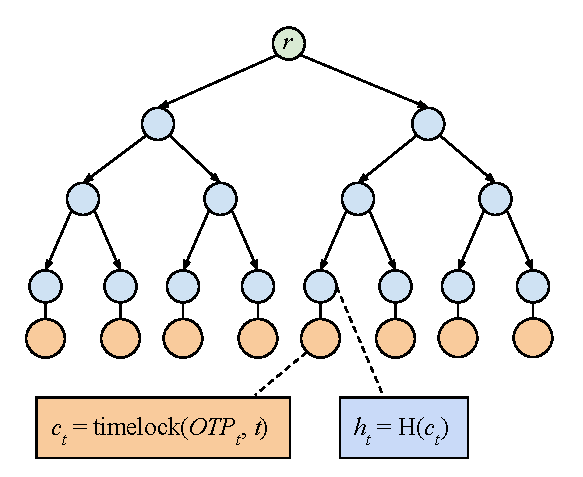
\includegraphics[width=\columnwidth,keepaspectratio]{figures/timelock-merkle.pdf}
    \else
        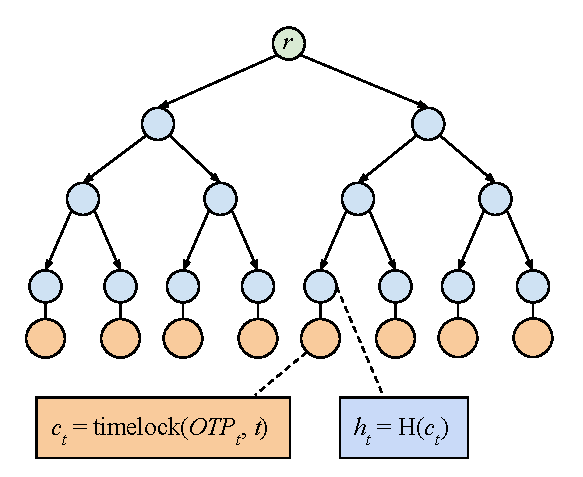
\includegraphics[width=0.7 \columnwidth,keepaspectratio]{figures/timelock-merkle.pdf}
    \fi
    \label{fig.merkle-otp}
\end{figure}

The honest party will always succeed in creating a valid spending transaction.
To see this, note that the party begins creating the commit transaction at time
$t - \ell - 2k$. Due to liveness, it becomes confirmed at block $t - 2k$ at most,
and so the check in Line~\ref{alg.otp.delay} will pass. The reveal transaction will
be called with the corresponding data and release the funds.

\import{./}{algorithms/alg.otp.tex}

To see why an adversary cannot create a valid spending transaction beyond random
guessing, we note that any adversary can either provide a commit transaction prior
to block $t - 2k$, or afterwards. If she provides a commit transaction
prior to it, then the timelock scheme will protect the secret, and so the spending
transaction will include a random OTP guess. On the other hand, if she provides a
commit transaction afterwards, it will not be accepted due to the time delay enforced
in Line~\ref{alg.otp.delay}. Consult the Analysis section for a more complete argument.

We remark that a standard time-based OTP cannot be used in this case, because the
chain, as a stochastic process, may have grown faster or slower than expected. The
OTP device must know the current height of the blockchain to be able to reveal the
correctly indexed OTP (which will reside at OTP index $|\chain| + \ell + 2k$).
One practical way to achieve this is to have the mobile
wallet (or a block explorer) display the current block height, which can then be
inputted by the user to the OTP application.

The OTP scheme can be used either as a single-factor or as a second factor combined
with a private key if desired. It is an effective second factor because,
if either, but not both, of the private key or the OTP device become compromised,
the wallet remains secure.

\import{./}{algorithms/alg.otp.external.tex}

One critical point of infrastructure is the online
computer to which the user inputs their OTP code. If that computer becomes
compromised, it can change the target address and amount that the user is
inputting and deplete the wallet. One practical mechanism to cut the user's losses
is to establish an hourly limit in the amount that can be spent by the wallet,
as illustrated in Algorithm~\ref{alg.otp}. In
such a case, the compromised computer can only steal the user's funds \emph{once},
and up to the specified hourly limit, before being detected.
